\chapter{Campo eléctrico atmosférico rápido}
\label{ch:background}



\begin{figure}[h!]
\begin{center}
\includegraphics[width=0.85\textwidth]{Figures/Diagrama_Rodilla.PNG}
\caption{Espectro de  rayos cósmicos diferencial en función de la energía. Se puede observar también los diferentes rangos de medición de los principales observatorios. Tomado de \cite{mollerach2018progress}}
\label{Diagrama_Rodilla}
\end{center}
\end{figure}


\section{Características de $\vec{E}$ rápido }
\section{Métodos de detección}
\section{Diseño del sensor de $\vec{E}$ rápido}
\subsection{Antena}
\subsection{Acondicionamiento de señal}

circuito de integración

Compensation of integrator time constants for electric field
measurements. Kohlmann. Leer y citar

respuesta en frecuencia del integrador


\subsection{Digitalización}
\subsection{Sistema de lectura}
FPGA, Memoria


\begin{figure}[h!]
\begin{center}
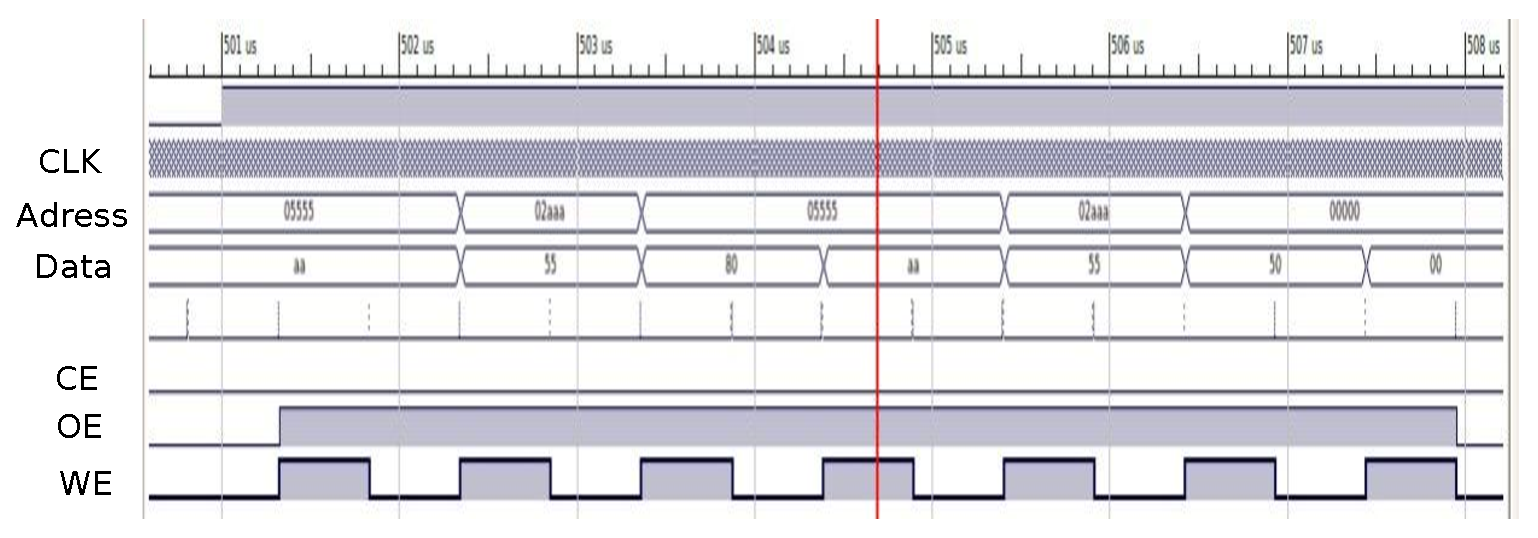
\includegraphics[width=1\textwidth]{Figures/VHDL.eps}
\caption[Estructura de un espectroscopio]{El electroscopio contiene en su interior 2 láminas delgadas de un conductor, éstas a su vez están conectadas a una varilla conductora con una esfera al final o parte plana. Cuando la esfera interactúa con una superficie cargada, las 2 láminas adquieren la misma carga de la varilla y por lo tanto se repelen, indicando la presencia de una carga. Imagen tomada de \cite{gordon1883physical}}
\label{ELectroscopio}
\end{center}
\end{figure}

\subsection{Trasmisión de datos}

Resumen características:

\begin{table}[ht]
\centering
  \caption{ Frontend and readout parameters}
  \begin{tabular}{ | c | c |}
    \hline
    Parameter & Value\\ \hline
    antenna  type & flat\\ \hline
    diameter [cm] & 20  \\ \hline
    recording length [ms] &  1000 \\ \hline
    pre-trigger [ms] & 200 \\ \hline
    post-trigger [ms] & 800 \\ \hline
    sampling frequency [Mhz] & 1 \\ \hline
    digitazion resolution [bits] & 12 \\ 
    \hline
  \end{tabular}
  \label{net}
\end{table}
Ref. Types of lightning discharges that abruptly terminate enhanced fluxes of energetic radiation and particles observed at ground level. Chilingarian. 2017


\section{Calibración}
\section{Primeras Mediciones}